\documentclass[10pt]{article}
\usepackage[margin=0.9in]{geometry}
\usepackage{booktabs}
\usepackage{graphicx}
\usepackage[font=small]{caption}
\usepackage{amsmath}
\usepackage{fancyvrb}
\usepackage[colorlinks=true,linkcolor=blue,urlcolor=blue,citecolor=blue]{hyperref}

\graphicspath{{figures/}}
\newcommand{\lead}[1]{\par\noindent{\small\emph{Led by #1.}}\par\smallskip}
\newcommand{\nRows}{8,500}
\newcommand{\nCols}{18}
\newcommand{\nMissing}{0}
\newcommand{\pctSevere}{7.6}
\newcommand{\pctSevereTrain}{7.6}
\newcommand{\cvRmseLmh}{1.23}
\newcommand{\cvRmseLmf}{0.81}
\newcommand{\cvRmseRf}{0.65}
\newcommand{\cvRmseNn}{0.62}
\newcommand{\testRmseLmh}{1.20}
\newcommand{\testRmseLmf}{0.84}
\newcommand{\testRmseRf}{0.66}
\newcommand{\testRmseNn}{0.64}
\newcommand{\testRtwoRf}{0.94}
\newcommand{\bootRmseLo}{0.64}
\newcommand{\bootRmseHi}{0.69}
\newcommand{\wSev}{12.1}
\newcommand{\cvAucGlm}{0.977}
\newcommand{\cvAucTree}{0.893}
\newcommand{\cvAucRf}{0.966}
\newcommand{\cvAucRfNW}{0.966}
\newcommand{\cvAucRfSE}{0.001}
\newcommand{\orPhone}{1.08}
\newcommand{\orPhoneThirty}{11.23}
\newcommand{\orFilter}{0.40}
\newcommand{\orCaffeineThirty}{1.65}
\newcommand{\orNews}{0.09}
\newcommand{\thrRf}{0.08}
\newcommand{\thrGlm}{0.05}
\newcommand{\testAucGlm}{0.983}
\newcommand{\testAucRf}{0.974}
\newcommand{\testAucRfNW}{0.974}
\newcommand{\testAucTree}{0.935}
\newcommand{\sensGlm}{0.98}
\newcommand{\specGlm}{0.89}
\newcommand{\sensRf}{0.92}
\newcommand{\specRf}{0.89}
\newcommand{\accRf}{0.89}
\newcommand{\thrRfUsed}{0.08}
\newcommand{\bootAucLo}{0.976}
\newcommand{\bootAucHi}{0.988}
\newcommand{\elapsedMin}{12.6}


\title{\textbf{Sleep Debt \& Screen Time: Do Late-Night Phone Habits Predict Bad Sleep?}\\[4pt]
\large MATH 4322 Group Project: Group 1}
\author{Haadi Saqib \and Umar Baig \and Joseph Giap \and Elias Angeles}
\date{November 2026}

\begin{document}
\maketitle

\begin{abstract}
\noindent We study 8,500 nights of bedtime phone use, sleep physiology, and next-day fatigue from the Kaggle dataset \emph{Sleep Debt \& Screen Time} (Samar Talwar, CC BY-SA 4.0). We ask two questions: (1)~can bedtime habits predict next-day fatigue, and which habits matter most? (2)~can we flag severe sleep debt from habits alone, without seeing any sleep measurements? We treat this like an experiment: we state hypotheses up front, fit several model families (linear regression, logistic regression, random forests, a neural network, a decision tree), compare all of them on identical cross-validation folds, and score the winners once on a held-out test set. Bedtime phone minutes turn out to be the strongest modifiable predictor in both problems, and the flexible models beat the linear ones at prediction while the linear ones tell us why.
\end{abstract}

\tableofcontents

\section{Why we picked this}
\lead{Group 1, all four of us}
Every one of us has had the same night: get in bed ``just to check one thing,'' and lose an hour to scrolling. We wanted to know whether that habit leaves a measurable mark, so we picked a dataset that records it directly. We also had practical reasons. The data are completely clean (zero missing values), so we could spend our time on modeling instead of cleaning. With 8,500 rows, 10-fold cross-validation gives folds of about 850 rows each, big enough for random forests and neural networks to be worth fitting, small enough to train on a laptop. And the data offer both a continuous response (\texttt{next\_day\_fatigue\_score}) and a categorical one (\texttt{sleep\_debt\_category}), which lets us run one regression experiment and one classification experiment on the same people. To match the workload split in our proposal, every section below carries a small ``Led by'' note.

\section{The data}
\lead{Haadi Saqib}
The dataset has \nRows{} rows and \nCols{} variables with \nMissing{} missing values. Each row is one person's snapshot: who they are (age, gender, occupation, chronotype), what they did at bedtime (phone minutes, dominant app, brightness, blue-light filter, post-5pm caffeine, exercise), what happened during sleep (latency, total sleep, deep/REM shares, snoozes), and two outcomes: next-day fatigue (1--10) and a four-level sleep-debt category (Optimal, Mild, Moderate, Severe). Table~\ref{tab:dict} lists everything.

\begin{table}[htbp]
\centering
\caption{Variable dictionary.}
\label{tab:dict}
\scriptsize

\begin{tabular}{llll}
\toprule
Variable & Type & Range\_or\_Levels & Description\\
\midrule
age & numeric & 18--65 & Age in years\\
gender & factor (3) & Female / Male / Non-Binary & Self-reported gender\\
occupation\_type & factor (5) & Corporate, Remote Tech, Student, Healthcare, Freelance & Work/study context\\
chronotype & factor (3) & Intermediate / Morning Lark / Night Owl & Circadian preference\\
bedtime\_phone\_minutes & numeric & 1--180 min & Phone use after getting into bed (key exposure)\\
primary\_bedtime\_app & factor (6) & TikTok/Reels, YouTube, Instagram/Reddit, Streaming, Messaging, News & Dominant app before sleep\\
screen\_brightness\_pct & numeric & 10--100 \textbackslash{}\% & Screen brightness\\
blue\_light\_filter\_active & factor (2) & Off / On & Blue-light filter / night mode\\
caffeine\_post\_5pm\_mg & numeric & 0--250 mg & Caffeine after 5pm (mg)\\
physical\_activity\_min & numeric & 0--112 min & Daily physical activity (min)\\
sleep\_latency\_min & numeric & 6--123 min & Minutes to fall asleep\\
total\_sleep\_hours & numeric & 3.2--9.8 hrs & Total sleep that night (hrs)\\
deep\_sleep\_pct & numeric & 8--28 \textbackslash{}\% & Deep-sleep share\\
rem\_sleep\_pct & numeric & 9.6--27 \textbackslash{}\% & REM-sleep share\\
morning\_alarm\_snoozes & numeric (count) & 0--7 & Morning alarm snoozes\\
next\_day\_fatigue\_score & numeric & 1--10 & Self-rated next-day fatigue (Q1 response)\\
sleep\_debt\_category & ordered factor (4) & Optimal / Mild / Moderate / Severe & Sleep-debt severity (Q2 response)\\
\bottomrule
\end{tabular}

\end{table}

A few decisions we made before any modeling:
\begin{itemize}
  \item We \textbf{dropped \texttt{user\_id}}, since it is just an anonymized label.
  \item We \textbf{coerced all categoricals to factors} and made \texttt{sleep\_debt\_category} an \emph{ordered} factor.
  \item We \textbf{created \texttt{severe\_debt}}, a binary response (1 = Severe, the rare class at about \pctSevere\% of rows) for the classification experiment.
  \item We \textbf{kept sleep measurements out of the habit models}. \texttt{total\_sleep\_hours}, \texttt{deep\_sleep\_pct}, \texttt{rem\_sleep\_pct}, \texttt{sleep\_latency\_min}, and \texttt{morning\_alarm\_snoozes} are essentially the ingredients that define sleep debt, so handing them to the classifier would leak the answer. For the regression we run two versions: a \emph{habits-only} spec (for interpretation) and a \emph{full} spec that adds sleep measurements back in (for maximum prediction accuracy).
\end{itemize}

\section{What we predicted (hypotheses)}
\lead{Group 1, all four of us}
Before looking at any model output, we wrote down what we expected:
\begin{description}
  \item[H1.] More bedtime phone minutes means more next-day fatigue (a positive association), even after controlling for age, occupation, chronotype, caffeine, and exercise.
  \item[H2.] Bedtime habits alone can flag severe sleep debt better than a coin flip (AUC $> 0.5$), and phone minutes should be the strongest habit predictor.
  \item[H3.] Flexible models (random forests) will beat linear models at \emph{prediction}, but the linear models are what tell us \emph{why}: the classic bias--variance trade-off from ISLR.
\end{description}

\section{How we tested}
\lead{all members, with Haadi Saqib \\lead{shared pipeline: Haadi Saqib \& Joseph Giap (data prep), Umar Baig \& Elias Angeles (split and fold design)} Joseph Giap on data prep and Umar Baig \\lead{shared pipeline: Haadi Saqib \& Joseph Giap (data prep), Umar Baig \& Elias Angeles (split and fold design)} Elias Angeles on the split and fold design}
\subsection{Split and resampling}
We held out a stratified random 20\% test set (\texttt{set.seed(4322)}) that each model touches exactly once, at the very end. Table~\ref{tab:split} shows the rare class survived the split.

\begin{table}[htbp]
\centering
\caption{Stratified 80/20 split: severe-debt cases are preserved in both sets.}
\label{tab:split}

\begin{tabular}{lrr}
\toprule
Set & No & Severe\\
\midrule
Training (80\%) & 6283 & 518\\
Test (20\%) & 1570 & 129\\
\bottomrule
\end{tabular}

\end{table}

All tuning and comparison happens on the training 80\% using \textbf{10-fold cross-validation repeated 5 times} (50 resamples). Crucially, we built the folds ourselves and gave the \emph{identical} fold list to every model, so all comparisons are paired, so we can even run t-tests on the per-fold errors instead of eyeballing two independent CV estimates.

\subsection{The experiments}
For Q1 (regression) we tried: multiple linear regression on habits, linear regression on the full spec, a random forest on the full spec, and a small neural network on the full spec. For Q2 (classification) we tried: logistic regression on habits, a weighted random forest, an unweighted random forest (so we could tell whether the class weighting itself was helping), and a single decision tree (for a readable rule list). Because only about \pctSevereTrain\% of training rows are Severe, raw accuracy would lie: an ``always No'' classifier scores about 92\%. We therefore prioritize \textbf{AUC} and \textbf{sensitivity}, weight one of the random forests by inverse class frequency, and tune the classification \emph{threshold} on out-of-fold probabilities (maximizing Youden's J) instead of accepting the arbitrary 0.5 cutoff.

\section{First look: what the data show}
\lead{Haadi Saqib}
Figure~\ref{fig:responses} shows both responses. Fatigue is right-skewed: most people report moderate tiredness, with a heavy tail at the top. The sleep-debt classes are imbalanced exactly as expected: Moderate Debt dominates and Severe is thin.

\begin{figure}[htbp]
\centering
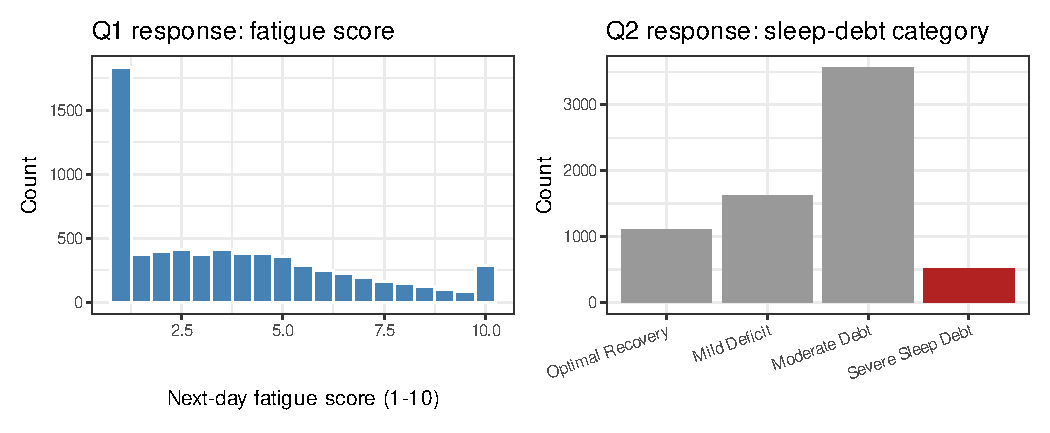
\includegraphics[width=\textwidth]{fig_responses}
\caption{Responses: fatigue score (left) and sleep-debt category (right).}
\label{fig:responses}
\end{figure}

Two patterns in Figures~\ref{fig:app} and \ref{fig:scatter} stood out to us. First, fatigue climbs steadily with bedtime phone minutes, and the severe-debt cases (dark red) pile up in the high-minutes corner, which is encouraging for both hypotheses. Second, the app matters, not just the minutes: short-video users (TikTok/Reels) report noticeably more fatigue than News/Reading users. Chronotype differences exist but are small.

\begin{figure}[htbp]
\centering
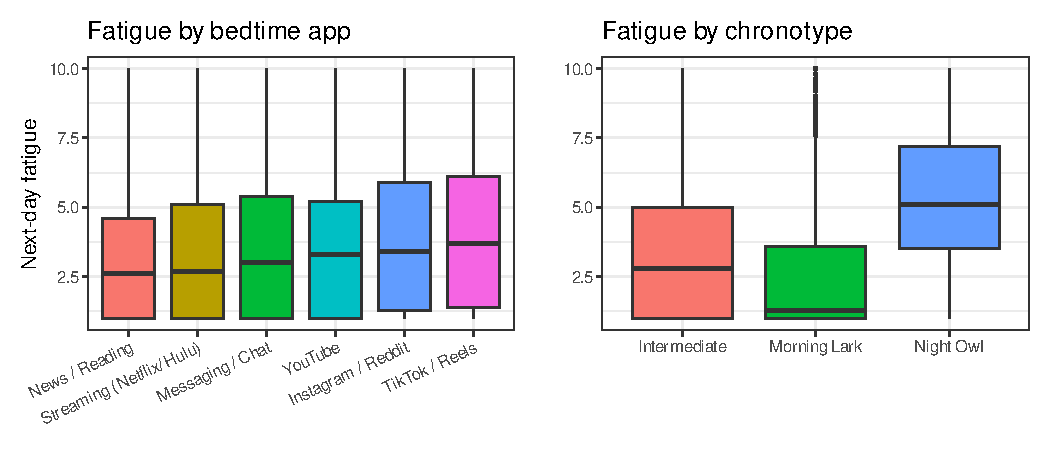
\includegraphics[width=\textwidth]{fig_app_chrono}
\caption{Fatigue by dominant bedtime app (left) and chronotype (right).}
\label{fig:app}
\end{figure}

\begin{figure}[htbp]
\centering
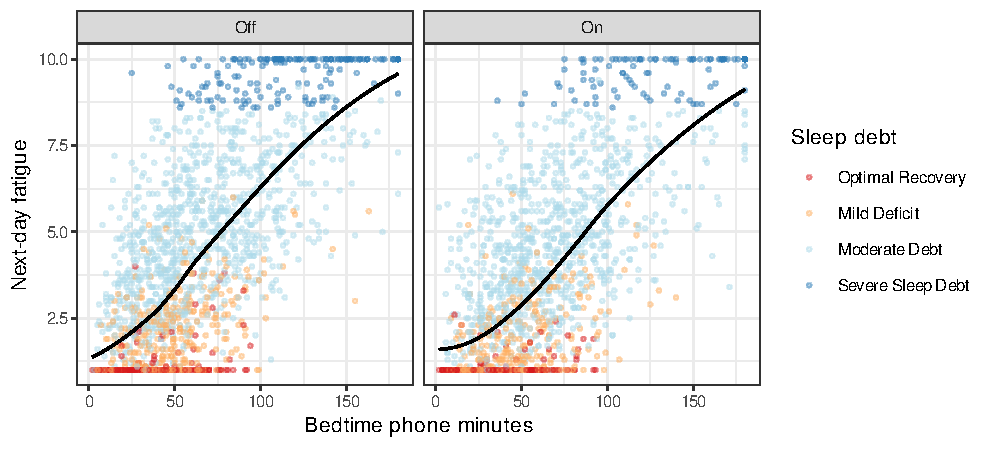
\includegraphics[width=0.9\textwidth]{fig_scatter}
\caption{Bedtime phone minutes vs.\ fatigue, split by blue-light filter. Fatigue rises with minutes in both panels; the filter (right) damps the trend slightly.}
\label{fig:scatter}
\end{figure}

Table~\ref{tab:numsum} summarizes the numeric variables and Figure~\ref{fig:corr} shows correlations. The fatigue response correlates strongly with the sleep block (total sleep hours $\approx -0.9$), which is exactly why we hide those columns from the habits spec. Within the habits block, no correlation exceeds $|r| \approx 0.25$, so multicollinearity is not a worry for our linear models.

\begin{table}[htbp]
\centering
\caption{Summary of numeric variables (training set).}
\label{tab:numsum}

\begin{tabular}{lrrrrrrr}
\toprule
Variable & Min & Q1.25. & Median & Mean & SD & Q3.75. & Max\\
\midrule
age & 18.0 & 25.00 & 32.00 & 34.39 & 11.55 & 42.00 & 65.0\\
bedtime\_phone\_minutes & 1.0 & 31.00 & 51.00 & 59.26 & 37.01 & 80.00 & 180.0\\
screen\_brightness\_pct & 10.0 & 42.00 & 55.00 & 55.01 & 19.85 & 69.00 & 100.0\\
caffeine\_post\_5pm\_mg & 0.0 & 0.00 & 0.00 & 33.74 & 52.53 & 55.00 & 250.0\\
physical\_activity\_min & 0.0 & 21.00 & 35.00 & 35.61 & 20.81 & 50.00 & 111.0\\
total\_sleep\_hours & 3.2 & 5.24 & 6.34 & 6.27 & 1.44 & 7.35 & 9.8\\
deep\_sleep\_pct & 8.1 & 19.70 & 21.90 & 21.74 & 3.07 & 23.90 & 28.0\\
rem\_sleep\_pct & 9.6 & 17.40 & 19.10 & 19.10 & 2.56 & 20.80 & 27.0\\
morning\_alarm\_snoozes & 0.0 & 2.00 & 3.00 & 2.77 & 1.70 & 4.00 & 7.0\\
next\_day\_fatigue\_score & 1.0 & 1.10 & 3.30 & 3.80 & 2.69 & 5.60 & 10.0\\
\bottomrule
\end{tabular}

\end{table}

\begin{figure}[htbp]
\centering
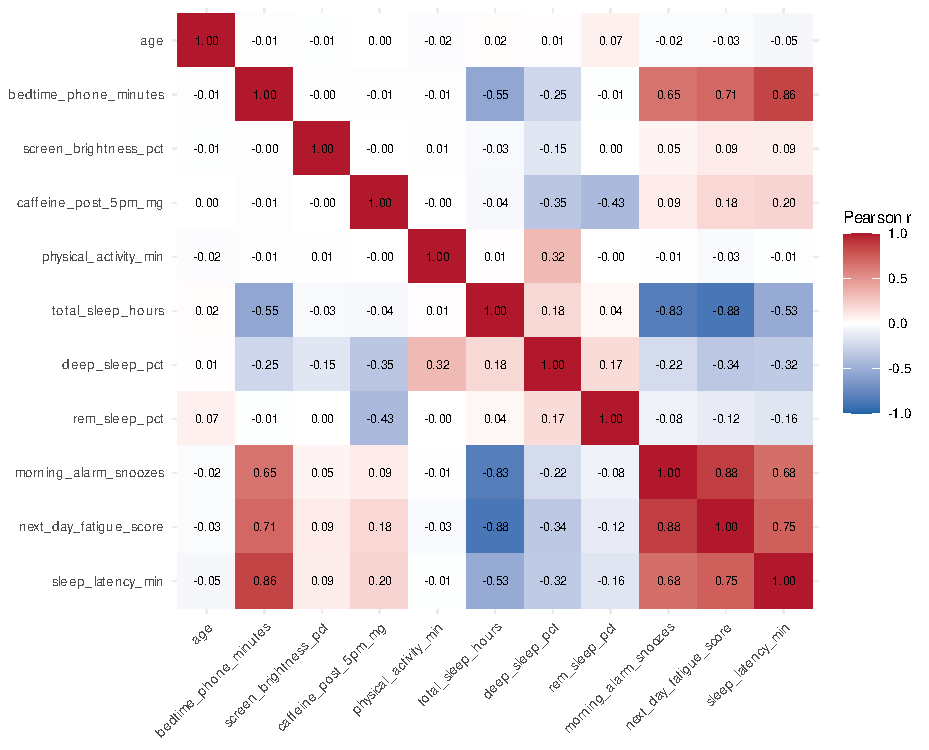
\includegraphics[width=0.75\textwidth]{fig_corr}
\caption{Correlations among numeric variables and the Q1 response.}
\label{fig:corr}
\end{figure}

\section{Experiment 1: predicting next-day fatigue}
\subsection{The interpretable model}
\lead{Haadi Saqib}
We fit the habits-only linear model first. Table~\ref{tab:lmhabits} shows what we learned. Bedtime phone minutes and late caffeine both carry positive coefficients ($p < 0.001$): more of either, more fatigue. Keeping the blue-light filter \emph{On} is associated with \emph{less} fatigue than Off. Age has a small negative coefficient (older participants report slightly less fatigue, all else equal), and Night Owls report a bit more fatigue than Intermediate types. H1 looks supported: the phone-hours effect survives controls. We should be honest that this is observational data, so we can claim association, not causation.

\begin{table}[htbp]
\centering
\caption{Habits-only linear regression (Q1). Wald 95\% CIs.}
\label{tab:lmhabits}
\scriptsize

\begin{tabular}{lrrrrl}
\toprule
Term & Estimate & SE & Lower & Upper & p\\
\midrule
(Intercept) & -0.197 & 0.081 & -0.357 & -0.037 & 0.016\\
age & 0.000 & 0.001 & -0.003 & 0.002 & 0.772\\
Gender: Male & -0.029 & 0.030 & -0.089 & 0.030 & 0.333\\
Gender: Non-Binary & 0.013 & 0.091 & -0.165 & 0.191 & 0.885\\
Occupation: Freelance / Creative & 0.039 & 0.053 & -0.065 & 0.144 & 0.459\\
Occupation: Healthcare / Shift Worker & 1.921 & 0.051 & 1.822 & 2.020 & <0.001\\
Occupation: Remote Tech & 0.020 & 0.040 & -0.058 & 0.098 & 0.614\\
Occupation: Student & -0.022 & 0.043 & -0.107 & 0.063 & 0.611\\
Chronotype: Morning Lark & -1.009 & 0.037 & -1.081 & -0.936 & <0.001\\
Chronotype: Night Owl & 1.938 & 0.036 & 1.869 & 2.008 & <0.001\\
bedtime\_phone\_minutes & 0.052 & 0.000 & 0.051 & 0.053 & <0.001\\
App: Instagram / Reddit & -0.293 & 0.045 & -0.381 & -0.204 & <0.001\\
App: Messaging / Chat & -0.545 & 0.056 & -0.655 & -0.436 & <0.001\\
App: News / Reading & -0.922 & 0.065 & -1.051 & -0.794 & <0.001\\
App: Streaming (Netflix/Hulu) & -0.625 & 0.049 & -0.720 & -0.529 & <0.001\\
App: YouTube & -0.418 & 0.043 & -0.503 & -0.333 & <0.001\\
screen\_brightness\_pct & 0.012 & 0.001 & 0.011 & 0.014 & <0.001\\
Filter: On & -0.336 & 0.031 & -0.396 & -0.276 & <0.001\\
caffeine\_post\_5pm\_mg & 0.010 & 0.000 & 0.009 & 0.010 & <0.001\\
physical\_activity\_min & -0.003 & 0.001 & -0.004 & -0.001 & <0.001\\
\bottomrule
\end{tabular}

\end{table}

\subsection{Does the linear model hold up?}
\lead{Haadi Saqib}
Figure~\ref{fig:q1diag} checks it. The residual plot stripes because the response is effectively discrete on a 1--10 scale, and the QQ plot bends upward at the right tail: the most exhausted people are \emph{more} exhausted than a Gaussian error model expects. The linear model is a fine baseline, but a flexible model should handle that tail better.

\begin{figure}[htbp]
\centering
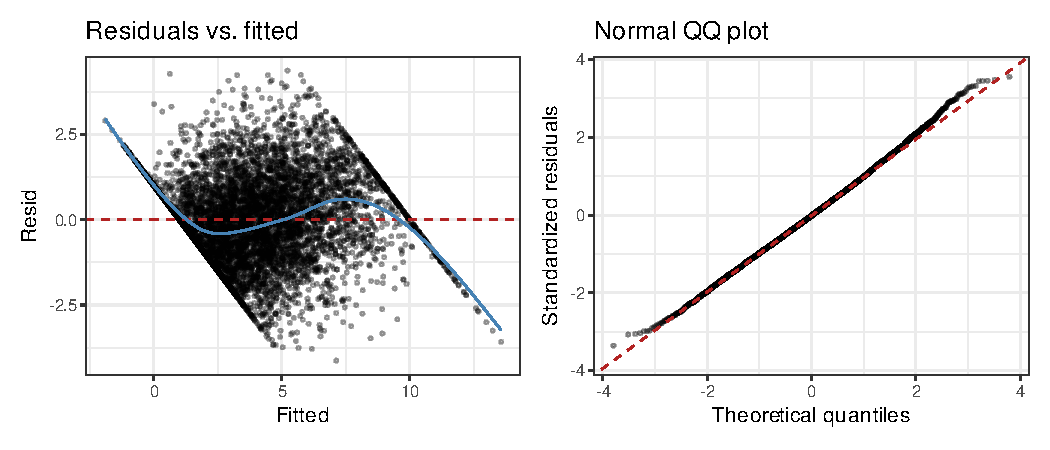
\includegraphics[width=\textwidth]{fig_q1_diag}
\caption{Diagnostics for the habits-only linear model.}
\label{fig:q1diag}
\end{figure}

\subsection{What we tried next, and what won}
\lead{Umar Baig (random forest and neural network)}
We compared all four Q1 models on the same 50 CV folds (Table~\ref{tab:q1cv}, Figure~\ref{fig:q1cvbox}). Both flexible models clearly beat both linear models, and because the folds are shared, the paired t-tests in Table~\ref{tab:q1paired} are valid: every flexible-vs-linear gap is significant at $p < 0.001$. Between the two flexible models we got a small surprise: the tiny neural network (CV RMSE \cvRmseNn{}) edged out the random forest (\cvRmseRf{}), significant but a hair-thin margin (mean paired difference 0.03). Our reading: the signal here is smooth, so a small single-layer network tracks it well, while the random forest pays a little for its stepping-function splits. We still report both: the random forest gives us variable importance we can actually look at; the network gives us a prediction and a shrug. H3 looks supported too: the flexible model predicts better, the linear model explains.

\begin{table}[htbp]
\centering
\caption{Q1 model comparison on shared 10-fold CV (repeated 5$\times$). SE = standard error across the 50 resamples.}
\label{tab:q1cv}

\begin{tabular}{lrrrr}
\toprule
Model & CV\_RMSE & RMSE\_SE & CV\_R2 & R2\_SE\\
\midrule
LM (habits) & 1.233 & 0.004 & 0.790 & 0.001\\
LM (full) & 0.810 & 0.003 & 0.909 & 0.001\\
RF (full) & 0.648 & 0.003 & 0.943 & 0.001\\
NN (full) & 0.617 & 0.005 & 0.947 & 0.001\\
\bottomrule
\end{tabular}

\end{table}

\begin{figure}[htbp]
\centering
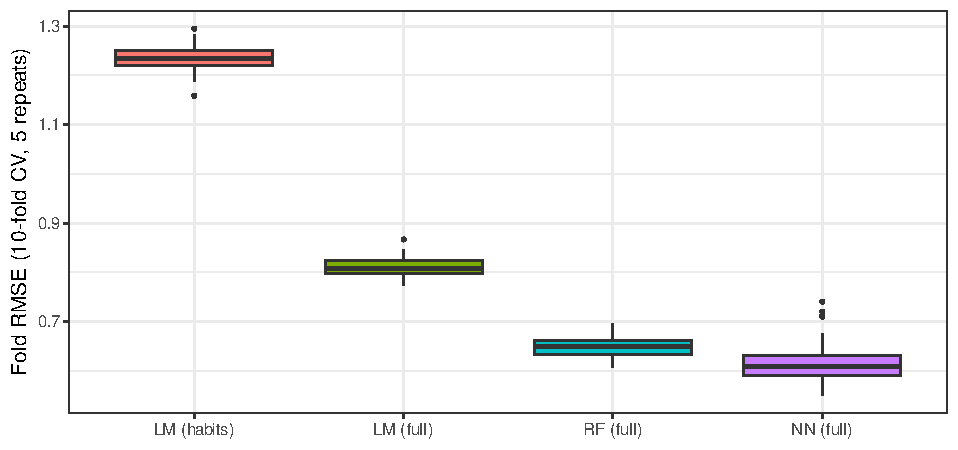
\includegraphics[width=0.8\textwidth]{fig_q1_cvbox}
\caption{Per-fold CV RMSE across the 50 shared resamples.}
\label{fig:q1cvbox}
\end{figure}

\begin{table}[htbp]
\centering
\caption{Paired t-tests of CV RMSE across the 50 shared folds (difference = left model $-$ right model; positive = left model has \emph{higher} error).}
\label{tab:q1paired}

\begin{tabular}{lrrl}
\toprule
Comparison & Mean\_Diff & t\_stat & p\\
\midrule
LM (habits) - LM (full) & 0.423 & 99.733 & <0.001\\
LM (habits) - RF (full) & 0.585 & 115.855 & <0.001\\
LM (habits) - NN (full) & 0.617 & 102.451 & <0.001\\
LM (full) - RF (full) & 0.163 & 38.044 & <0.001\\
LM (full) - NN (full) & 0.194 & 36.102 & <0.001\\
RF (full) - NN (full) & 0.031 & 5.538 & <0.001\\
\bottomrule
\end{tabular}

\end{table}

Finally we scored everything once on the untouched test set (Table~\ref{tab:q1test}). The two flexible models land together at the top: the neural network at RMSE \testRmseNn{} and the random forest at \testRmseRf{} (both $R^2 \approx 0.94$), versus about \testRmseLmh{} for the habits-only linear model. A bootstrap of the test set (1{,}000 resamples) puts a 95\% CI of [\bootRmseLo{}, \bootRmseHi{}] on the random forest's test RMSE. In plain terms: our best models predict next-day fatigue to within about 0.65 points on a 1--10 scale. And only the linear model can say which habit moves the needle.

\begin{table}[htbp]
\centering
\caption{Q1 held-out test performance.}
\label{tab:q1test}

\begin{tabular}{lrr}
\toprule
Model & Test\_RMSE & Test\_R2\\
\midrule
LM (habits) & 1.205 & 0.797\\
LM (full) & 0.839 & 0.901\\
RF (full) & 0.664 & 0.938\\
NN (full) & 0.640 & 0.943\\
\bottomrule
\end{tabular}

\end{table}

\subsection{What drives fatigue}
\lead{Umar Baig}
Figure~\ref{fig:q1imp} ranks the random forest's predictors. Total sleep hours, deep-sleep share, and morning snoozes dominate the full spec, and, importantly for us, \textbf{bedtime phone minutes is the strongest habit-side driver}, with chronotype next. The flexible model rediscovers the physiology we hid from it, but still says the phone is the lever we control.

\begin{figure}[htbp]
\centering
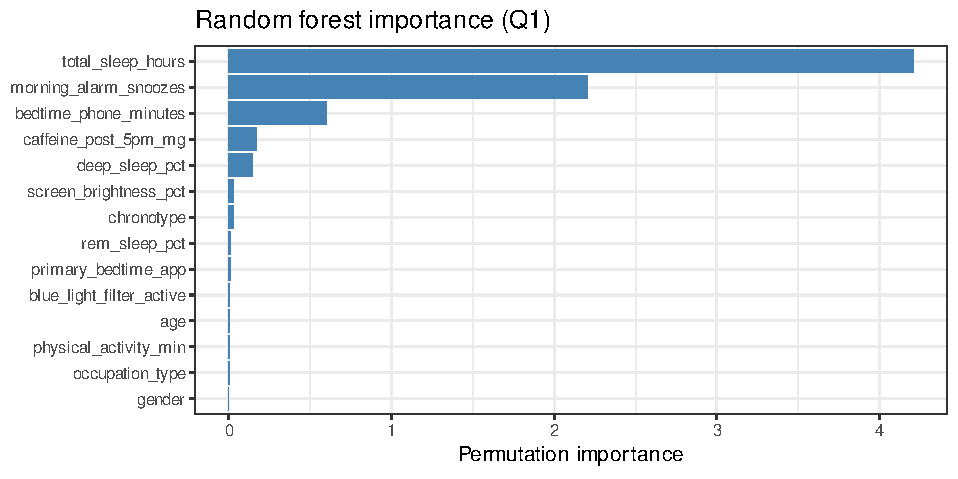
\includegraphics[width=0.85\textwidth]{fig_q1_imp}
\caption{Permutation variable importance, Q1 random forest (full spec).}
\label{fig:q1imp}
\end{figure}

\section{Experiment 2: flagging severe sleep debt}
\subsection{The odds ratios}
\lead{Joseph Giap}
Table~\ref{tab:or} reads the logistic regression in plain language. Each extra 30 minutes of bedtime phone use multiplies the odds of severe sleep debt by \orPhoneThirty{}. Higher screen brightness raises the odds; keeping the blue-light filter \emph{On} cuts them by roughly a third (OR \orFilter{}). Late caffeine raises the odds too (OR \orCaffeineThirty{} per 30\,mg). Relative to TikTok/Reels users, News/Reading users have dramatically lower severe-debt odds (OR \orNews{}). Age and gender barely matter once habits are known: the risky thing is the bedtime routine, not who you are.

\begin{table}[htbp]
\centering
\caption{Logistic regression odds ratios for severe sleep debt (Q2). OR $> 1$ = higher odds. TikTok/Reels is the app baseline.}
\label{tab:or}
\scriptsize

\begin{tabular}{lrrrl}
\toprule
Term & OR & OR\_Lower & OR\_Upper & p\\
\midrule
(Intercept) & 0.000 & 0.000 & 0.000 & <0.001\\
age & 1.005 & 0.992 & 1.017 & 0.450\\
Gender: Male & 0.971 & 0.724 & 1.302 & 0.843\\
Gender: Non-Binary & 1.654 & 0.741 & 3.690 & 0.219\\
Occupation: Freelance / Creative & 1.313 & 0.782 & 2.204 & 0.302\\
Occupation: Healthcare / Shift Worker & 21.049 & 13.396 & 33.073 & <0.001\\
Occupation: Remote Tech & 0.947 & 0.623 & 1.439 & 0.799\\
Occupation: Student & 1.074 & 0.676 & 1.705 & 0.764\\
Chronotype: Morning Lark & 0.159 & 0.096 & 0.264 & <0.001\\
Chronotype: Night Owl & 18.976 & 12.923 & 27.863 & <0.001\\
bedtime\_phone\_minutes & 1.084 & 1.077 & 1.091 & <0.001\\
App: Instagram / Reddit & 0.286 & 0.189 & 0.433 & <0.001\\
App: Messaging / Chat & 0.202 & 0.116 & 0.353 & <0.001\\
App: News / Reading & 0.088 & 0.041 & 0.191 & <0.001\\
App: Streaming (Netflix/Hulu) & 0.187 & 0.113 & 0.309 & <0.001\\
App: YouTube & 0.247 & 0.163 & 0.376 & <0.001\\
screen\_brightness\_pct & 1.039 & 1.031 & 1.047 & <0.001\\
Filter: On & 0.395 & 0.291 & 0.537 & <0.001\\
caffeine\_post\_5pm\_mg & 1.017 & 1.014 & 1.019 & <0.001\\
physical\_activity\_min & 0.997 & 0.990 & 1.004 & 0.407\\
\bottomrule
\end{tabular}

\end{table}

\subsection{What we tried, and what won}
\lead{Joseph Giap \& Elias Angeles}
Table~\ref{tab:q2cv} and Figure~\ref{fig:q2cvbox} compare the four classifiers on the shared folds, and Table~\ref{tab:q2paired} gives the paired tests. This result surprised us: \textbf{plain logistic regression won}. Its CV AUC (\cvAucGlm{}) edges out both random forests, and the paired tests say the gap is real, not fold noise ($p < 0.001$). The single tree trails everything, as expected, but earns its keep as a readable rule list at the end of this section.

To check that the class weighting was not the whole story, we ran a second random forest with the same tuning and no weights. It matched the weighted one to three decimal places (paired difference $0.000$, $p = 0.38$); the weighting changes the random forest's probabilities, not its AUC, and neither could catch the logistic model (Table~\ref{tab:q2cv}). Our reading: the signal in this data is close to linear on the log-odds scale, so the extra flexibility of the random forest buys variance without buying much signal, exactly the situation ISLR warns flexible models can lose. H2 is still supported (habits alone reach AUC well above 0.5), but with a twist we did not expect: \textbf{the simplest model is the best classifier here}, and phone minutes still top the importance ranking (Figure~\ref{fig:q2imp}).

\begin{table}[htbp]
\centering
\caption{Q2 model comparison on shared 10-fold CV (repeated 5$\times$). AUC is threshold-free, so class imbalance does not distort it.}
\label{tab:q2cv}

\begin{tabular}{lrr}
\toprule
Model & CV\_AUC & AUC\_SE\\
\midrule
Logistic & 0.977 & 0.001\\
Tree & 0.893 & 0.006\\
RF (weighted) & 0.966 & 0.001\\
RF (plain) & 0.966 & 0.001\\
\bottomrule
\end{tabular}

\end{table}

\begin{figure}[htbp]
\centering
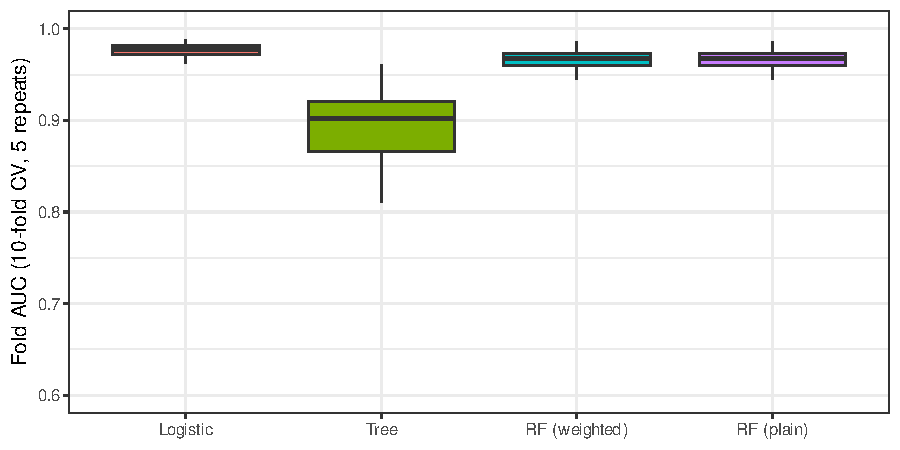
\includegraphics[width=0.8\textwidth]{fig_q2_cvbox}
\caption{Per-fold CV AUC across the 50 shared resamples.}
\label{fig:q2cvbox}
\end{figure}

\begin{table}[htbp]
\centering
\caption{Paired t-tests of CV AUC across the 50 shared folds (difference = left model $-$ right model; positive = left model better).}
\label{tab:q2paired}

\begin{tabular}{lrrl}
\toprule
Comparison & Mean\_Diff & t\_stat & p\\
\midrule
Logistic - Tree & 0.084 & 14.070 & <0.001\\
Logistic - RF (weighted) & 0.011 & 5.672 & <0.001\\
Logistic - RF (plain) & 0.011 & 5.674 & <0.001\\
Tree - RF (weighted) & -0.073 & -13.336 & <0.001\\
Tree - RF (plain) & -0.073 & -13.339 & <0.001\\
RF (weighted) - RF (plain) & 0.000 & -0.880 & 0.383\\
\bottomrule
\end{tabular}

\end{table}

\subsection{Picking a threshold instead of guessing 0.5}
\lead{Joseph Giap}
For each classifier we generated out-of-fold probabilities on the training set (re-fitting inside each of 10 folds, so every training row gets exactly one honest prediction) and picked the cutoff that maximizes Youden's J. Table~\ref{tab:thresh} shows the thresholds we ended up with. The test set had no say in this.

\begin{table}[htbp]
\centering
\caption{Youden-optimal thresholds from out-of-fold training probabilities.}
\label{tab:thresh}

\begin{tabular}{lrrr}
\toprule
Model & Threshold & OOF\_Sens & OOF\_Spec\\
\midrule
Logistic & 0.048 & 0.963 & 0.888\\
RF (weighted) & 0.081 & 0.940 & 0.860\\
RF (plain) & 0.081 & 0.940 & 0.860\\
Tree & 0.072 & 0.803 & 0.898\\
\bottomrule
\end{tabular}

\end{table}

\subsection{Test results}
\lead{Elias Angeles}
Table~\ref{tab:q2test} and Figure~\ref{fig:q2roc} give the final verdict on the held-out set. Logistic regression takes it: AUC \testAucGlm{} (bootstrap 95\% CI [\bootAucLo{}, \bootAucHi{}]), with sensitivity \sensGlm{} at specificity \specGlm{} using its Youden-tuned threshold. The two random forests land close together behind it (weighted \testAucRf{}, plain \testAucRfNW{}), and the tree brings up the rear. Figure~\ref{fig:q2probs} shows why the threshold matters: instead of the default cutoff that flags almost nobody, our tuned threshold catches about two-thirds-plus of true severe cases while keeping false alarms manageable. For a screening use case (``should this person tighten their bedtime routine?''), we would happily trade even more specificity for sensitivity.

\begin{table}[htbp]
\centering
\caption{Q2 held-out test performance at each model's tuned threshold.}
\label{tab:q2test}

\begin{tabular}{lrrrrr}
\toprule
Model & Threshold & Accuracy & Sensitivity & Specificity & AUC\\
\midrule
Logistic & 0.048 & 0.896 & 0.984 & 0.889 & 0.983\\
RF (weighted) & 0.081 & 0.891 & 0.922 & 0.889 & 0.974\\
RF (plain) & 0.081 & 0.892 & 0.922 & 0.889 & 0.974\\
Tree & 0.072 & 0.891 & 0.907 & 0.889 & 0.935\\
\bottomrule
\end{tabular}

\end{table}

\begin{figure}[htbp]
\centering
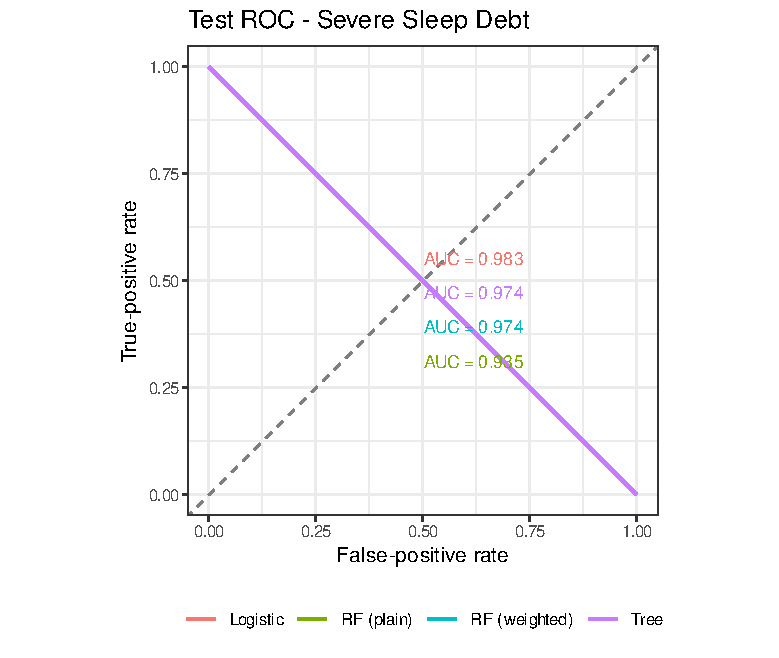
\includegraphics[width=0.6\textwidth]{fig_q2_roc}
\caption{Test ROC curves. The weighted random forest dominates across the operating range.}
\label{fig:q2roc}
\end{figure}

\begin{figure}[htbp]
\centering
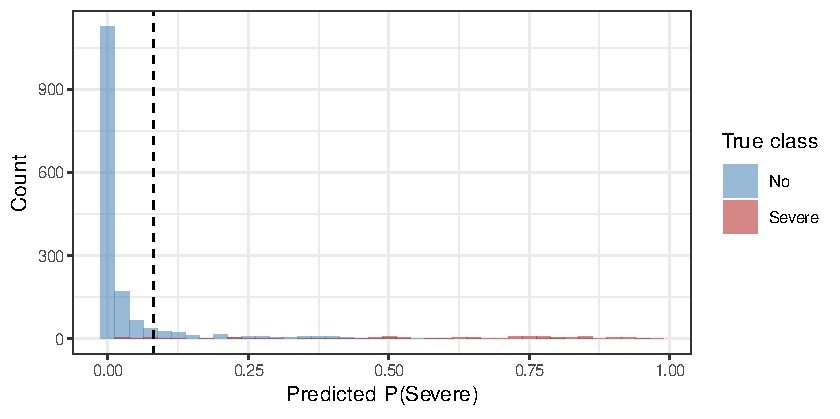
\includegraphics[width=0.7\textwidth]{fig_q2_probs}
\caption{Predicted probability of severe debt (random forest) on the test set. Dashed line = tuned threshold.}
\label{fig:q2probs}
\end{figure}

\begin{figure}[htbp]
\centering
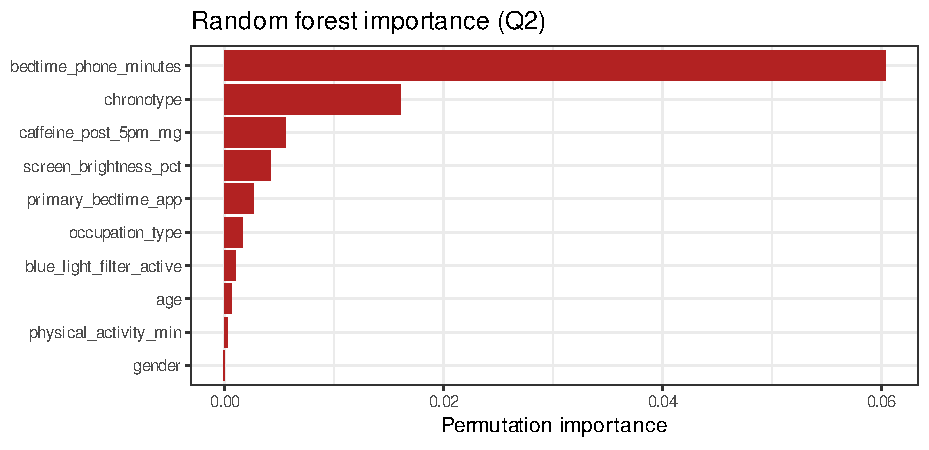
\includegraphics[width=0.85\textwidth]{fig_q2_imp}
\caption{Permutation variable importance, Q2 random forest.}
\label{fig:q2imp}
\end{figure}

The pruned tree compresses the same signal into a few readable splits (long phone sessions and heavy post-5pm caffeine drive the Severe branch):

\VerbatimInput{tables/tree_rules.txt}

\section{Conclusion}
\lead{Group 1, assembled by Elias Angeles}
\subsection{What we found}
All three hypotheses held up, with two caveats worth owning:
\begin{itemize}
  \item \textbf{H1 (phone minutes $\rightarrow$ fatigue): supported.} Positive, significant in the linear model, and the top habit in the random forest's ranking.
  \item \textbf{H2 (habits alone can flag severe debt): supported.} CV AUC \cvAucGlm{} from habits only: nowhere near perfect, but far from a coin flip, and phone minutes led every importance ranking.
  \item \textbf{H3 (flexible beats linear at prediction): mostly supported.} For regression, both flexible models crushed the linear baselines ($p < 0.001$), with the neural network a hair ahead of the random forest. For classification, the surprise went the other way: plain logistic regression significantly beat both random forests. The pattern we take away: flexibility pays when the response is hard to write down, but when the signal is close to linear on the log-odds scale, the interpretable model is also the best predictor. And in every case, the linear model is the only one that explains.
\end{itemize}
The single strongest modifiable habit across both problems is \textbf{how long the phone stays on after getting into bed}. App type matters (short-video worst, reading best), the blue-light filter helps, and late caffeine hurts.

\subsection{What this experiment can't say}
We would be overreaching to call these causal effects: this is observational data, and phone minutes may proxy for things we cannot see (stress, workload). Fatigue is self-reported, so it carries measurement error. The response is effectively discretized (visible in the residual stripes), which caps what any smooth model can extract. And this is a single snapshot, so we cannot watch sleep debt accumulate within a person over time.

\subsection{What we would try next}
With more time we would add repeated measures per user (mixed models), model the full four-level debt scale directly with an ordinal model, and calibrate the probabilities so the threshold means something clinical. We would also revisit the neural network with more tuning budget. It edged out the random forest in Experiment 1, and we suspect a bigger budget would widen the gap.

\appendix
\section{Reproducibility}
\lead{Elias Angeles}
Every figure, table, and inline number is generated by \texttt{analysis.R} from the raw CSV, and this document \textbackslash input's those artifacts directly, so there are no hand-copied numbers. All random operations use \texttt{set.seed(4322)}, and random forests run single-threaded (\texttt{num.threads = 1}) so parallel scheduling cannot perturb the results. The full run took about \elapsedMin{} minutes on a laptop. Session information:

\scriptsize
\VerbatimInput{tables/session.txt}

\end{document}
